\chapter{Implementierungsstrategie}\label{ch:implementierung}


\section{Schrittweise Umsetzung}\label{sec:schrittweise-umsetzung}

Die Umsetzung der Maßnahmen folgt den etablierten Phasen einer \gls{erp}-Anpassung: Projektplanung, Systemkonfiguration, Datenmigration/ -bereinigung, Testphase, Schulung und Go-Live \parencite[Folie~322 und 350]{coletta2026_0206}. Insgesamt ist sie auf sechs Monate ausgelegt (Abbildung~\ref{fig:implementierungsplan}). Nach dem Detailkonzept (P1) laufen die Stammdatenbereinigung (P2) und das Customizing des Kreditmanagements (P3) parallel. Die Umstellung der Fakturierungsläufe (P4) ist bewusst früh terminiert, weil sie mit geringem Aufwand die größte Liquiditätswirkung entfaltet („Quick Win“, Abbildung~\ref{fig:liegezeiten}). Es folgen der Gutschriften-Workflow (P5), Integrationstests und Schulungen (P6) sowie Go-Live mit Hypercare-Phase (P7). Die Planung nutzt die klassischen Instrumente Projektstrukturplan, Meilensteine und Gantt-Diagramm \parencite[Folie~238]{coletta2026_2804}.

\begin{figure}[!htb]
\centering
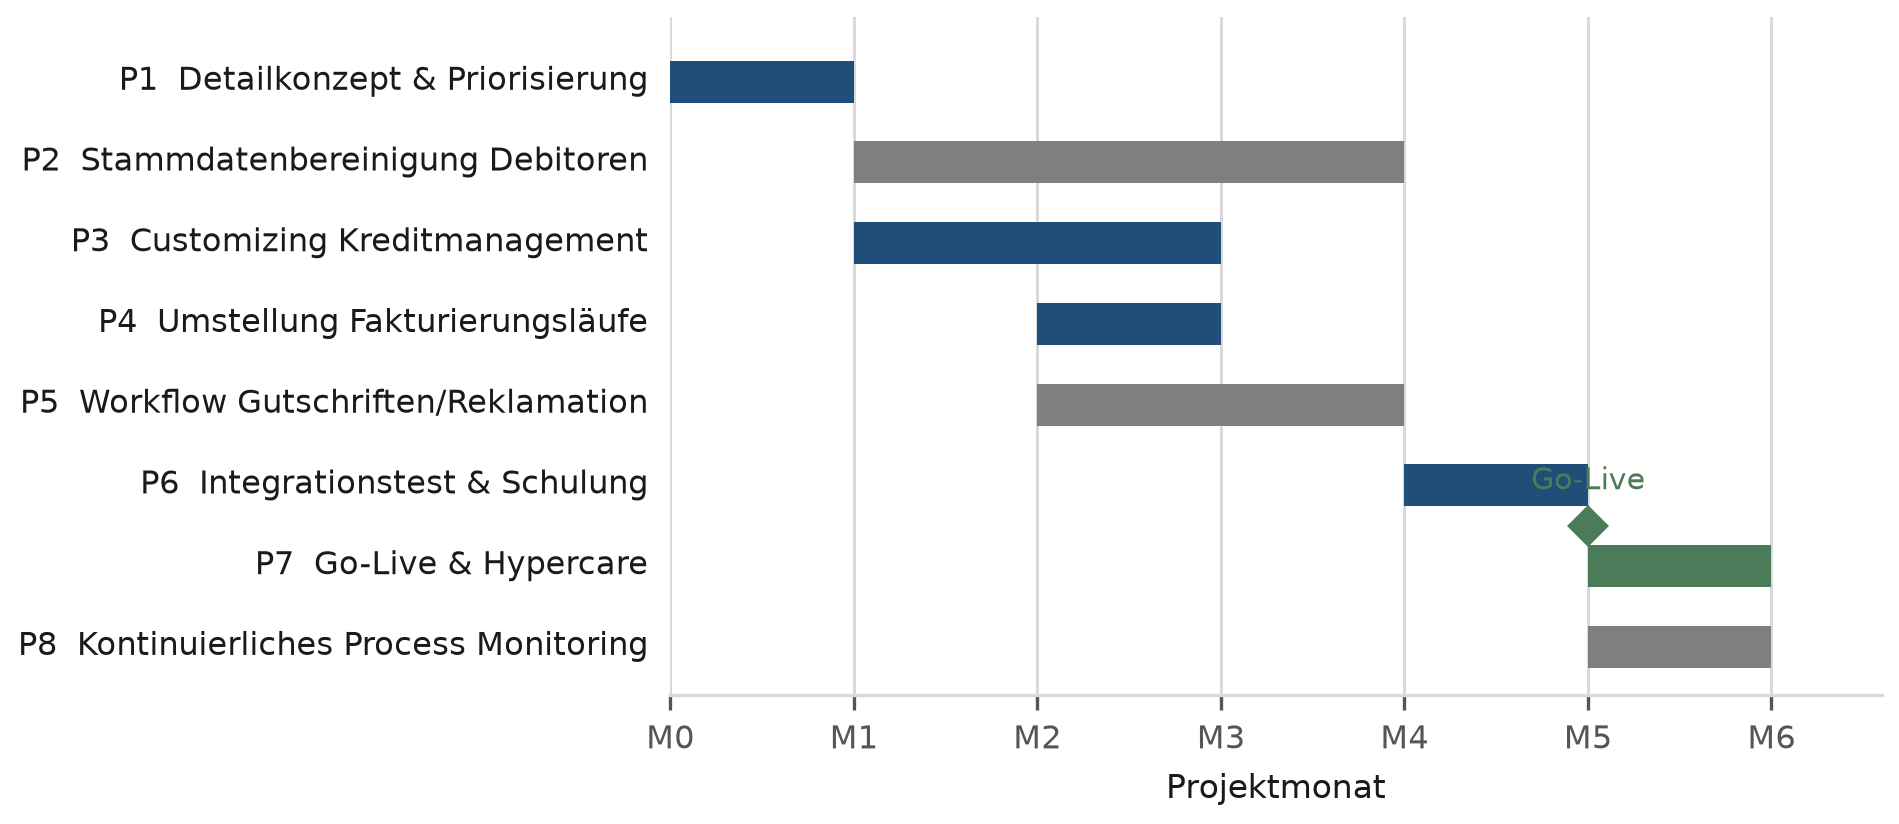
\includegraphics[width=\textwidth,height=0.36\textheight,keepaspectratio]{figures/image7.png}
\caption{Implementierungsplan über sechs Monate (Quelle: eigene Darstellung)}\label{fig:implementierungsplan}
\end{figure}

Ein iteratives, phasenweises Vorgehen ist auch aus Risikosicht geboten. Statt alle sechs Maßnahmen gleichzeitig produktiv zu setzen, werden sie nacheinander eingeführt und ihre Wirkung jeweils über das Prozessmonitoring gemessen, bevor die nächste folgt. So lässt sich etwa bei der automatisierten Kreditprüfung (M1) in einem Parallellauf beobachten, ob die neuen Regeln zu viele Aufträge blockieren oder umgekehrt Risikofälle durchlassen, und die Schwellenwerte können nachjustiert werden, bevor die manuelle Prüfung vollständig abgelöst wird. Dieses Vorgehen entspricht dem empfohlenen Phased Rollout und reduziert das Risiko, dass eine fehlerhafte Einstellung den gesamten \gls{o2c}-Prozess stört \parencite[Folie~337]{coletta2026_0206}. Inhaltlich gliedert sich das Vorhaben damit in eine Vorbereitungsphase (Detailkonzept und Priorisierung anhand der gemessenen Kennzahlen), eine Umsetzungsphase (parallele Stammdatenbereinigung und Customizing mit dem Fakturalauf als frühem Quick Win) und eine Stabilisierungsphase (Integrationstest, Schulung, Go-Live und Hypercare). Der Übergang von einer Phase zur nächsten ist jeweils an ein messbares Ergebnis geknüpft, etwa eine gesunkene Sperrquote im Parallellauf. Die Gesamtdauer von sechs Monaten ergibt sich dabei weniger aus dem technischen Aufwand der einzelnen Einstellungen, der überschaubar ist, als aus der Stammdatenbereinigung, den Testzyklen und der notwendigen Eingewöhnung der Anwender.

\section{Zeitplan und notwendige Ressourcen}\label{sec:zeitplan-ressourcen}

Für die Testphase sind Integrations-, User-Acceptance- und Regressionstests mit realistischen Testdaten vorgesehen \parencite[Folie~333 und 335]{coletta2026_0206}. Personell erfordert das Vorhaben eine interne Projektleitung (ca. 0,3 \gls{vzae}), je einen Key-User aus Vertrieb, Versand und Debitorenbuchhaltung (je ca. 0,2 \gls{vzae}), externe \gls{sd}-/\gls{fscm}-Beratung (ca. 25 Personentage) sowie die \gls{it} für Berechtigungen und Hintergrundjobs. Die externen Kosten lassen sich auf Basis marktüblicher Beratungstagessätze grob auf 60.000 bis 80.000 \euro{} schätzen. Dem stehen im modellierten Szenario rund 1.950 eingesparte Klärungsstunden pro Jahr (ca. 1,2 \gls{vzae}) sowie eine um mehrere Tage verkürzte Zeitspanne bis zur Rechnungsstellung gegenüber, die die Forderungslaufzeit unmittelbar senkt. Nach der \gls{roi}-Logik der Vorlesung amortisiert sich das Vorhaben unter diesen Annahmen bereits im ersten Jahr \parencites[Folie~343 ff.]{coletta2026_0206}[Folie~386 ff.]{coletta2026_0906}. Nach dem Go-Live werden Erfolgskriterien als Post-Go-Live-Metriken definiert und in der Hypercare-Phase proaktiv überwacht \parencite[Folie~337 und 341]{coletta2026_0206}, unmittelbar über das Prozessmonitoring aus Kapitel~\ref{sec:modifikationen-monitoring} mit den Kennzahlen aus Anhang A3.

Die Testphase verdient dabei besondere Aufmerksamkeit, weil die Maßnahmen tief in den erlöswirksamen Prozess eingreifen. Neben den funktionalen Integrationstests sind Regressionstests der angrenzenden Prozesse in Beschaffung, Bestandsführung und Debitorenbuchhaltung vorzusehen, und die neuen Kreditregeln sind an einem repräsentativen Ausschnitt historischer Aufträge zu erproben, um Fehlsperren zu vermeiden. Erst nach erfolgreichem User-Acceptance-Test durch die Key-User erfolgt der Go-Live.

Wirtschaftlich ist das Vorhaben auch unter konservativen Annahmen tragfähig. Den einmaligen externen Kosten stehen wiederkehrende Effekte gegenüber, nämlich eingesparte Klärungsstunden, eine kürzere Forderungslaufzeit und eine höhere Liefertermintreue. Weil die Liquiditätswirkung der täglichen Fakturierung sofort und ohne laufende Kosten eintritt, während die Beratungskosten nur einmalig anfallen, verschiebt sich das Kosten-Nutzen-Verhältnis bereits im ersten Jahr deutlich ins Positive. Entscheidend für die Belastbarkeit dieser Rechnung ist, dass die zugrunde liegenden Ist-Werte aus der Analyse gemessen und nicht geschätzt sind, sodass die erwarteten Einsparungen an konkreten, nachprüfbaren Kennzahlen festgemacht werden können.

\section{Risikobewertung und Managementstrategien}\label{sec:risikobewertung}

Dass \gls{erp}-nahe Projekte ihre Zeitpläne häufig überschreiten, ist empirisch gut belegt. Nur rund 21 Prozent der \gls{erp}-Implementierungen bleiben im Zeitplan. Als Hauptgründe gelten organisatorische Probleme, unrealistische Zeitpläne und Scope-Ausweitung \parencite[Panorama Consulting/Statista, zit.\ nach][Folie~211 und 213]{coletta2026_2804}. Tabelle~\ref{tab:risikomatrix} bewertet die wichtigsten Risiken und hinterlegt Gegenmaßnahmen. Hervorzuheben ist das Datenschutzrisiko, das beim Übergang von synthetischen auf reale Event-Logs entsteht. Reale Logs enthalten Benutzerkennungen und erlauben Leistungs- und Verhaltensauswertungen, Betriebsrat und Datenschutzbeauftragte sind daher früh einzubinden, und die Analysen sind auf pseudonymisierte, nicht personenbezogene Auswertungen zu beschränken.

\begin{table}[!htb]
\centering
\caption{Risikomatrix der Implementierung}\label{tab:risikomatrix}
\small
\begin{tabularx}{\textwidth}{@{}Y l l Y@{}}
\toprule
\textbf{Risiko} & \textbf{Eintritt} & \textbf{Auswirkung} & \textbf{Gegenmaßnahme} \\
\midrule
Datenqualität schlechter als angenommen (Stammdaten) & hoch & mittel & frühe Testextraktion, Bereinigung priorisieren, Puffer in P2 \\
Zu scharfe Kreditregeln blockieren Aufträge /\allowbreak{} zu laxe erhöhen Forderungsausfälle & mittel & hoch & Pilotbetrieb mit Parallellauf, Schwellenwerte iterativ justieren, Ausnahmeliste \\
Akzeptanz: Mitarbeitende fühlen sich durch Prozessdaten überwacht (reale Logs) & mittel & hoch & Pseudonymisierung, Betriebsvereinbarung, transparente Kommunikation der Ziele \\
Scope-Ausweitung (weitere Prozesse „auch noch schnell“) & mittel & mittel & Change-Request-Verfahren, Priorisierung nach Nutzwert \\
Wissensabfluss nach Beratungsende & niedrig & mittel & Dokumentation, Key-User-Schulung, Betreuungsvereinbarung \\
\bottomrule
\end{tabularx}
\end{table}

Neben diesen sachlichen Risiken ist das Veränderungsmanagement entscheidend, weil die Maßnahmen etablierte Arbeitsweisen ablösen. Die Umstellung von der manuellen auf die automatisierte Kreditfreigabe etwa entzieht der Debitorenbuchhaltung eine gewohnte Kontrollaufgabe und muss durch frühzeitige Einbindung, transparente Kommunikation der Ziele und Schulung begleitet werden. Gerade weil Process Mining das tatsächliche Verhalten sichtbar macht, ist der offene Umgang mit den Ergebnissen, verbunden mit der klaren Zusage, die Auswertung nicht zur individuellen Leistungskontrolle zu nutzen, eine Voraussetzung für die Akzeptanz im Team.

